\documentclass[12pt, twoside]{article}
% \documentclass[12pt, twoside]{article}
\usepackage[letterpaper, margin=1in, headsep=0.2in]{geometry}
\setlength{\headheight}{0.6in}
%\usepackage[english]{babel}
\usepackage[utf8]{inputenc}
\usepackage{microtype}
\usepackage{amsmath}
\usepackage{amssymb}
%\usepackage{amsfonts}
\usepackage[nomessages]{fp} %\FPeval{\var-name}{2*sin(pi/6)}
\usepackage{siunitx} %units in math. eg 20\milli\meter
\usepackage{yhmath} % for arcs, overparenth command
\usepackage{tikz} %graphics
\usetikzlibrary{quotes, angles, arrows, arrows.meta}
\usepackage{graphicx} %consider setting \graphicspath{{images/}}
\usepackage{parskip} %no paragraph indent
\usepackage{enumitem}
\usepackage{multicol}
\usepackage{venndiagram}

\usepackage{fancyhdr}
\pagestyle{fancy}
\fancyhf{}
\renewcommand{\headrulewidth}{0pt} % disable the underline of the header
\raggedbottom
\hfuzz=2mm %suppresses overfull box warnings

\usepackage{hyperref}
\usepackage{float}

\title{Algebra 2}
\author{Chris Huson}
\date{September 2024}

\fancyhead[LE]{\thepage}
\fancyhead[RO]{\thepage \\ First and last name: \hspace{2.5cm} \,\\ Section: \hspace{2.5cm} \,}
\fancyhead[LO]{BECA/Huson/Precalculus: Sequences \\* 19 September 2024}

\begin{document}
\subsubsection*{1.12 Homework: Algebra practice }
\begin{enumerate}

\begin{multicols}{2}
      \item Given $f(x)=3x$. Simplify $f(2)$.
      \item Find $g(x)=2x-7$ for $x=9$.
\end{multicols} \vspace{3cm}

\item Given $\displaystyle h(x)=\frac{5x+7}{11}$. Evaluate the expression $h(3)$. \vspace{3cm}

Combine like terms
\begin{multicols}{2}
\item $x^2+2x -6 -2x^2-x+14$
\item $5(a^2-2a +3) -2(2a^2-5a-4)$
\end{multicols} \vspace{4cm}

Solve for the value of $x$. Check your solution.
\begin{multicols}{2}
\item   $3x+6=12$
\item   $2(3x-4)=3(x+2)+1$ 
\end{multicols} \vspace{4.5cm}

\newpage
Solve for the value of $x$. Check your solution.
\begin{multicols}{2}
\item   $x-6=\frac{1}{3}(6-9x)$
\item   $1=\frac{1}{3}x-10$
\end{multicols} \vspace{6cm}

\item Plot the points on the grid and draw a line through them.
  \begin{multicols}{2}
    What is the slope and $y$-intercept of the line?
    \begin{flushleft}
      \begin{tabular}{|c|r|}
      \hline
      $x$ & $f(x)$\\
      \hline
      -1 & -3 \\
      \hline
      0 & -1 \\
      \hline
      1 & 1 \\
      \hline
      2 & 3 \\
      \hline
      3 & 5 \\
      \hline
      \end{tabular}
    \end{flushleft}
    \columnbreak

    \begin{center} %4 quadrant regents grid
    \begin{tikzpicture}%[scale=.635]
      \draw [help lines] (-3,-4) grid (4,6);
      \draw [thick, ->] (-3.2,0) -- (4.4,0) node [below right] {$x$};
      \draw [thick, ->] (0,-4.2)--(0,6.4) node [left] {$y$};
    \end{tikzpicture}
    \end{center}
  \end{multicols}


\end{enumerate}
\end{document}
